\documentclass[a5paper,headsepline,titlepage,10pt]{scrbook}
\usepackage[a5paper,backref]{hyperref}
\usepackage[papersize={148.5mm,215mm},twoside,bindingoffset=0.5cm,hmargin={2cm,2cm},
				vmargin={2cm,2cm},footskip=1.1cm,driver=dvipdfm]{geometry}
\usepackage{graphicx}
\usepackage{fancyhdr}
\usepackage{palatino}
\usepackage{marvosym}
\usepackage[bahasa]{babel}

\renewcommand{\footrulewidth}{0.5pt}
\lhead[\fancyplain{}{\thepage}]%
      {\fancyplain{}{\rightmark}}
\rhead[\fancyplain{}{\leftmark}]%
      {\fancyplain{}{\thepage}}
\pagestyle{fancy}
\lfoot[\emph{Satrio dan Nanda}]{}
\rfoot[]{\emph{Misa Syukur Perkawinan}}
\cfoot{}

\makeatletter
\newcommand{\judul}[1]{%
  {\parindent \z@ \centering \normalfont
    \interlinepenalty\@M \Large \bfseries #1\par\nobreak \vskip 20\p@ }}
\newcommand{\subjudul}[1]{%
  {\parindent \z@ \normalfont
    \interlinepenalty\@M \bfseries #1\par\nobreak \vskip 20\p@ }}
\newcommand{\lagu}[1]{%
  {\parindent \z@ \normalfont
    \interlinepenalty\@M \bfseries \emph{#1}\par\nobreak \vskip 20\p@ }}

\renewenvironment{description}
               {\list{}{\labelwidth\z@ \itemindent-\leftmargin
                        \let\makelabel\descriptionlabel}}
               {\endlist}
\renewcommand*\descriptionlabel[1]{\hspace\labelsep 
                                \normalfont\bfseries #1 }
    

\makeatother

\newcommand{\BU}[1]{\begin{itemize} \item[U:] #1 \end{itemize}}
\newcommand{\BI}[1]{\begin{itemize} \item[I:] #1 \end{itemize}}
\newcommand{\BP}[1]{\begin{itemize} \item[P:] #1 \end{itemize}}
\newcommand{\ultah}{0 }
\newcommand{\suami}{Adrianus Satrio Adinugroho }
\newcommand{\istri}{Maria Hernanda Ika Kristiani }
\newcommand{\orangtua}{Ibu Ignatia Sudarmini }
\newcommand{\romo}{Gregorius Heliarko, SJ }
\hyphenation{ba-gi-mu}
\hyphenation{di-se-rah-kan}
\hyphenation{me-la-lui}
\hyphenation{ka-nak}
\hyphenation{ka-re-na}
\hyphenation{ber-ka-ta}
\hyphenation{te-ta-pi}
\hyphenation{per-ka-win-an}
\hyphenation{pa-tut}
\hyphenation{me-lu-hur-kan}
\hyphenation{ber-nya-nyi}
\hyphenation{di-tum-pah-kan}
\hyphenation{pe-ngam-pun-an}
\hyphenation{ber-a-da}
\hyphenation{kau-lim-pah-kan}
\hyphenation{ke-bang-kit-an-Nya}
\hyphenation{per-ka-ta-an}
\hyphenation{pa-sang-kan-lah}
\hyphenation{DA-RAH-KU}
\hyphenation{ke-na-ik-kan-nya}
\hyphenation{per-sem-bah-an}
\hyphenation{per-se-ku-tu-an}
\hyphenation{Tu-han}
\hyphenation{mem-per-si-ap-kan}
\hyphenation{ke-lu-ar-ga-ke-lu-ar-ga}
\hyphenation{ke-lu-ar-ga}
\hyphenation{Te-ri-ma-lah}
\hyphenation{a-kan}
\hyphenation{ME-NGE-NANG-KAN}
\hyphenation{mengem-bang-kan}
\hyphenation{me-nga-gum-kan}
\hyphenation{o-rang}
\hyphenation{ke-se-la-mat-an}
\hyphenation{ke-se-la-mat-an-Mu}


\usepackage[bahasa]{babel}
\selectlanguage{bahasa}

%\topmargin=-0.5in
%\textheight=8in
\title{MISA \\SYUKUR PERKAWINAN}
\author{

\includegraphics[scale=1]{ill044}\\
\suami \\dan \\\istri \\
\\ 
oleh Romo \romo} 
\date{14 Juni 2014}
\begin{document}

\maketitle
%\thispagestyle{empty}

\judul{RITUS PEMBUKA}

\lagu{Lagu pembukaan}

\subjudul{Tanda Salib}
\BI{Dalam nama Bapa dan Putera dan Roh Kudus}
\BU{Amin}

\subjudul{Salam Pembuka}
\BI{Rahmat Tuhan kita Yesus Kristus, cinta kasih Allah, dan persekutuan Roh Kudus beserta kita}
\BU{Sekarang dan selama-lamanya}

\subjudul{Pengantar}
\BI{Bapak, Ibu, dan Saudara-saudara pada kesempatan ini kita diundang keluarga \orangtua  untuk  bersyukur atas pernikahan anaknya tercinta.

Keluarga ini bersyukur atas perjalanan hidup yang tidak pernah lepas dari berkat dan rahmat Tuhan. Berkat dan rahmat itu sungguh-sungguh nyata dan dirayakan oleh keluarga ini terutama melalui segala kebaikan yang telah mereka terima dari saudara sekalian.

Misa syukur ini secara khusus dipersembahkan bagi kita semua sebagai ungkapan terima kasih atas segala kebaikan yang senantiasa mengalir di dalam keluarga ini.}

\subjudul{Tobat}
\BI{Marilah kita hening sejenak untuk mempersiapkan diri dalam perayaan syukur ini sambil menyadari bahwa kita sering melupakan kebaikan Tuhan dan enggan mewartakan dan mewujudkan kebaikan tersebut melalui pikiran, perkataan, dan perbuatan kita.}

\BI{Saya mengaku}

\BU{Kepada Allah yang Maha Kuasa dan kepada saudara sekalian bahwa saya telah berdosa dengan pikiran dan perkataan, dengan perbuatan dan kelalaian. Saya berdosa, saya berdosa, saya sungguh berdosa. Oleh sebab itu saya mohon kepada Santa Perawan Maria, kepada Para Malaikat dan orang kudus dan kepada saudara sekalian, supaya mendoakan saya kepada Allah Tuhan kita.}

\BI{Semoga Allah Yang Maha Kuasa mengasihi kita, mengampuni dosa kita dan menghantar kita ke hidup yang kekal.}

\BU{Amin}

\lagu{Tuhan Kasihanilah Kami}

\subjudul{Doa Pembukaan}

\BI{Marilah kita berdoa,

Allah, pencipta dan penebus kami, Engkau menghendaki agar pria dan wanita membangun keluarga yang bahagia. Kedua pasang suami isteri, para hambaMu ini, baru saja memasuki bahtera perkawinan. Berkatilah cinta kasih mereka supaya tahan uji dalam untung dan malang, dan anugerahkanlah mereka keturunan yang dapat dibanggakan. Demi Kristus, Putera-Mu, Tuhan dan pengantara kami, yang bersatu dengan Dikau dan Roh Kudus, hidup dan berkuasa kini dan sepanjang masa. Amin.}

\BU{Amin}

\judul{LITURGI SABDA}

\subjudul{Bacaan pertama: Kolose 3:12-21}

\BP{\emph{Pembacaan dari Surat Pertama Rasul Paulus kepada Umat di Kolose.}

Karena itu, sebagai orang-orang pilihan Allah yang dikuduskan dan dikasihi-Nya, kenakanlah bel
as kasihan, kemurahan, kerendahan hati, kelemahlembutan dan kesabaran.
Sabarlah kamu seorang terhadap yang lain, dan ampunilah seorang akan yang lain apabila yang seorang menaruh dendam terhadap yang lain, sama seperti Tuhan telah mengampuni kamu, kamu perbuat jugalah demikian.
Dan di atas semuanya itu: kenakanlah kasih, sebagai pengikat yang mempersatukan dan menyempurnakan.
Hendaklah damai sejahtera Kristus memerintah dalam hatimu, karena untuk itulah kamu telah dipanggil menjadi satu tubuh. Dan bersyukurlah.

Hendaklah perkataan Kristus diam dengan segala kekayaannya di antara kamu, sehingga kamu dengan segala hikmat mengajar dan menegur seorang akan yang lain dan sambil menyanyikan mazmur, dan puji-pujian dan nyanyian rohani, kamu mengucap syukur kepada Allah di dalam hatimu.
Dan segala sesuatu yang kamu lakukan dengan perkataan atau perbuatan, lakukanlah semuanya itu dalam nama Tuhan Yesus, sambil mengucap syukur oleh Dia kepada Allah, Bapa kita.

Hai isteri-isteri, tunduklah kepada suamimu, sebagaimana seharusnya di dalam Tuhan.
Hai suami-suami, kasihilah isterimu dan janganlah berlaku kasar terhadap dia.
Hai anak-anak, taatilah orang tuamu dalam segala hal, karena itulah yang indah di dalam Tuhan.
Hai bapa-bapa, janganlah sakiti hati anakmu, supaya jangan tawar hatinya.

Demikianlah sabda Tuhan.
}

\BU{Syukur kepada Allah.}

\lagu{Lagu antar bacaan}

\lagu{Bait Pengantar Injil}

\BI{Alleluia, Alleluia, Alleluia} 

\BU{Alleluia, Alleluia, Alleluia} 

\BI{Jika kita saling mengasihi, Allah tinggal di dalam kita dan cinta kasih Allah di dalam kita menjadi sempurna.} 
	
\BU{Alleluia, Alleluia, Alleluia} 

\subjudul{Bacaan Injil: Mat 2:13-15,19-23}

\BI{Tuhan sertamu}

\BU{Dan sertamu juga}

\BI{Inilah Injil Yesus Kristus menurut Santo Mateus}

\BU{Dimuliakanlah Tuhan}

\BI{
Setelah orang-orang majus itu berangkat, nampaklah malaikat Tuhan kepada Yusuf dalam mimpi dan berkata: "Bangunlah, ambillah Anak itu serta ibu-Nya, larilah ke Mesir dan tinggallah di sana sampai Aku berfirman kepadamu, karena Herodes akan mencari Anak itu untuk membunuh Dia."
Maka Yusufpun bangunlah, diambilnya Anak itu serta ibu-Nya malam itu juga, lalu menyingkir ke Mesir,
dan tinggal di sana hingga Herodes mati. Hal itu terjadi supaya genaplah yang difirmankan Tuhan oleh nabi: "Dari Mesir Kupanggil Anak-Ku."

Setelah Herodes mati, nampaklah malaikat Tuhan kepada Yusuf dalam mimpi di Mesir, katanya:
"Bangunlah, ambillah Anak itu serta ibu-Nya dan berangkatlah ke tanah Israel, karena mereka yang hendak membunuh Anak itu, sudah mati."
Lalu Yusufpun bangunlah, diambilnya Anak itu serta ibu-Nya dan pergi ke tanah Israel.

Tetapi setelah didengarnya, bahwa Arkhelaus menjadi raja di Yudea menggantikan Herodes, ayahnya, ia takut ke sana. Karena dinasihati dalam mimpi, pergilah Yusuf ke daerah Galilea.
Setibanya di sana iapun tinggal di sebuah kota yang bernama Nazaret. Hal itu terjadi supaya genaplah firman yang disampaikan oleh nabi-nabi, bahwa Ia akan disebut: Orang Nazaret.

Demikianlah injil Tuhan
}

\BU{Terpujilah Kristus}

\subjudul{Homili}


\subjudul{Aku Percaya}

\subjudul{Doa Umat}

\BI{Saudara-saudara, marilah berdoa bagi kedua saudara kita ini, bagi sanak saudara mereka, dan bagi seluruh umat Allah, khususnya yang tinggal di wilayah ini.}

\BP{Ya Tuhan, pencipta dan pembimbing manusia, lindungilah suami istri yang mulai memasuki jenjang perkawinan ini. Persatukanlah mereka dalam cinta kasih sejati. 

Marilah kita mohon...}

\BU{Kabulkanlah doa kami ya Tuhan}

\BP{Ya Tuhan, Pemberi damai dan kesejahteraan, dampingilah suami istri ini. Berilah hasil melimpah kepada pekerjaan mereka, dan jagalah sanak saudara mereka dalam kerukunan. 

Marilah kita mohon...}

\BU{Kabulkanlah doa kami ya Tuhan}


\BP{Ya Tuhan, pelindung dan penyelamat kami. Tunjukkanlah belas kasih-Mu kepada kami semua dan limpahilah  keluarga-keluarga kami dengan kurnia-Mu. 


Marilah kita mohon...}

\BU{Kabulkanlah doa kami ya Tuhan}

\BP{Ya Tuhan, gembala dan penghibur umat beriman, bahagiakanlah arwah nenek moyang keluarga-keluarga ini yang sudah menghadap hadirat-Mu. Terimalah mereka dalam perjamuan abadi di surga. 


Marilah kita mohon...}

\BU{Kabulkanlah doa kami ya Tuhan}

\BP{Ya Tuhan, sumber kebaikan dan cinta kasih, semoga suami istri ini tumbuh dalam cinta, dan hidup dalam kerukunan serta damai selama hayat dikandung badan. 


Marilah kita mohon...}

\BU{Kabulkanlah doa kami ya Tuhan}

\BI{Ya Tuhan, peliharalah saudara-saudari kami ini dalam cinta-Mu, bantulah dan
tuntunlah mereka seumur hidup serta kabulkanlah doa-doa kami. Demi Kristus Tuhan
dan Pengantara kami.}

\BU{Amin}

\judul{LITURGI EKARISTI}

\subjudul{Persiapan Persembahan}

\lagu{Lagu persembahan}

\BI{Kami memuji Engkau, Ya Bapa, Allah semesta alam. Sebab dari kemurahan-Mu kami menerima roti dan anggur yang kami persembahkan ini. Inilah hasil dari bumi dan usaha manusia yang bagi kami akan menjadi santapan rohani.}

\BU{Terpujilah Allah selama-lamanya}

\BI{Berdoalah saudara-saudara, supaya persembahan kita ini diterima oleh Allah, Bapa Yang Mahakuasa.}

\BU{Semoga persembahan ini diterima demi kemuliaan Tuhan dan keselamatan kita serta seluruh umat Allah yang kudus.}

\subjudul{Doa Persiapan Persembahan:}

\BI{Marilah berdoa,

Allah Bapa di surga, terimalah ucapan puji dan syukur keluarga ini sebagai persembahan yang harum mewangi. Sebab hanya puji dan syukur yang mereka berikan atas segala kebaikan yang senantiasa Kau limpahkan kepada keluaraga ini melalui orang-orang di sekitar keluarga ini. Dengan pengantaraan Kristus, Tuhan kami.}

\BU{Amin.}

\subjudul{Prefasi}

\BI{Tuhan sertamu}
\BU{Dan sertamu juga}
\BI{Marilah mengarahkan hati kepada Tuhan}
\BU{Sudah kami arahkan}
\BI{Marilah bersyukur kepada Tuhan Allah kita}
\BU{Sudah layak dan sepantasnya}
\BI{Sungguh layak dan sepantasnya, ya Bapa yang Kudus, Allah yang kekal dan kuasa, bahwa di manapun juga kami senantiasa bersyukur kepada-Mu dengan pengantaraan Kristus, Tuhan kami. Sebab kami yang seharusnya binasa karena dosa telah ditebus oleh kemenangan Kristus atas maut, dan karena kemurahan serta kebaikan-Mu kami dipanggil untuk hidup bersama Dia, Tuhan dan pengantara kami. Maka, kami selalu meluhurkan Dikau bersama seluruh laskar surgawi yang tak henti-hentinya memuji keagungan-Mu sambil bersukaria dan bernyanyi:}

\lagu{Kudus}

\subjudul{Doa Syukur Agung II}

\BI{Sungguh kuduslah Engkau ya Bapa. Segala ciptaan patut memuji Engkau. Sebab dengan pengantaraan Putra-Mu, Tuhan kami Yesus Kristus, dan dengan daya kekuatan Roh Kudus Engkau menghidupkan dan menguduskan segala sesuatu. Tak henti-hentinya Engkau menghimpun umat-Mu, sehingga dari terbitnya matahari sampai terbenamnya di seluruh bumi dipersembahkan kurban yang murni untuk memuliakan nama-Mu. Maka kami mohon ya Bapa sudilah menguduskan persembahan ini dengan Roh-Mu agar bagi kami menjadi tubuh ($\dagger$) dan darah Putra-Mu terkasih Tuhan kami, Yesus Kristus yang menghendaki kami merayakan misteri ini.

Sebab pada malam ia dikhianati, Yesus mengambil roti, Ia mengucap syukur dan memuji Dikau, memecahkan-mecahkan roti itu dan memberikannya kepada murid-murid-Nya seraya berkata:

TERIMALAH DAN MAKANLAH! INILAH TUBUHKU, YANG DISERAHKAN BAGIMU!

Demikian pula sesudah perjamuan, Yesus mengambil piala. Sekali lagi Ia mengucap syukur dan memuji Dikau, lalu memberikan piala itu kepada murid-murid-Nya seraya berkata:

TERIMALAH DAN MINUMLAH INILAH PIALA DARAHKU, DARAH PERJANJIAN BARU DAN KEKAL, YANG DITUMPAHKAN BAGIMU DAN BAGI SEMUA ORANG DEMI PENGAMPUNAN DOSA. LAKUKANLAH INI UNTUK MENGENANGKAN DAKU!}

\lagu{Anamnese}

\BI{Bapa, kami mengenangkan sengsara Putra-Mu, yang menyelamatkan, kebangkitan-Nya yang mengagumkan, dan kenaikkan-Nya ke surga. Sambil mengharapkan kedatangan-Nya kembali, dengan penuh syukur kami mempersembahkan kepada-Mu kurban yang hidup dan kudus ini. Kami mohon, pandanglah persembahan Gereja-Mu ini dan indahkanlah kurban yang telah mendamaikan kami dengan Dikau ini.

Semoga kami disempurnakan oleh-Nya menjadi suatu persembahan abadi bagi-Mu, agar kami pantas mewarisi kebahagiaan surgawi bersama para pilihan-Mu, terutama bersama Santa Perawan Maria, Bunda Allah, para rasul-Mu yang kudus, dan para martir-Mu yang jaya, dan bersama semua orang kudus yang selalu mendampingi dan menolong kami.

Ya Bapa, semoga berkat korban yang mendamaikan ini, damai sejahtera dan keselamatan semakin dirasakan oleh dunia.

Kuatkanlah Iman dan cinta kasih Gereja-Mu yang kini masih berziarah di bumi ini bersama hamba-Mu, Paus Benedictus XVI dan Uskup kami \dots \dots, serta semua uskup, para imam, diakon serta semua pelayan umat, dan seluruh umat kesayangan-Mu. Dengarkanlah doa-doa umat-Mu yang berhimpun di sini. Demi kerahiman dan kasih setia-Mu, ya Bapa, persatukanlah semua anak-Mu di mana pun mereka berada.

Sudilah pula menganugerahkan kebahagiaan abadi kepada semua yang telah berpulang ke hadirat-Mu, saudara-saudara kami seiman, dan semua orang lain yang hidupnya berkenan pada-Mu. Pada waktu itu, Engkau menghapus setiap tetes air mata kami, karena dengan memandang Engkau, ya Bapa, kami akan serupa dengan Dikau sepanjang masa dan tak henti-hentinya memuji Dikau.

Kami berharap, agar bersama mereka kami pun menikmati kemuliaan-Mu selama-lamanya, dengan pengantaraan Kristus, Tuhan kami. Sebab melalui Dialah Engkau melimpahkan segala yang baik kepada dunia.

Dengan pengantaraan Kristus, bersama Dia dan dalam Dia, bagi-Mu Allah Bapa Yang Maha Kuasa, dalam persekutuan dengan Roh Kudus, segala hormat dan kemuliaan, sepanjang segala masa. Amin.}

\subjudul{Bapa Kami}

\subjudul{Doa Damai}

\BI{Ya Bapa, dengan penuh kasih Engkau telah menciptakan dan menyertai keluarga-keluarga supaya menjadi sarana dan tanda bagi karya kesela-matan-Mu.

Berkatilah kami semua serta seluruh keluarga kami dengan kasih sayang, kegembiraan, kerukunan, dan kedamaian.

Tuhan Yesus Kristus, jangan memperhitungkan dosa kami, tetapi perhatikanlah iman gereja-Mu, dan restuilah kami supaya hidup bersatu dengan rukun sesuai dengan kehendak-Mu. Sebab Engkaulah pengantara kami, kini dan sepanjang masa.}

\BU{Amin.}

\subjudul{Salam Damai}

\BI{Semoga Damai Tuhan kita Yesus Kristus beserta kita}

\BU{Sekarang dan selama-lamanya.}

\lagu{Anak Domba Allah}

\subjudul{Persiapan Komuni}

\BI{Inilah Anak domba Allah yang menghapus dosa dunia. Berbahagialah kita yang diundang ke perjamuan-Nya}
\BU{Ya Tuhan, saya tidak pantas Engkau datang pada saya. Tetapi bersabdalah saja, maka saya akan sembuh.}

\lagu{Lagu Komuni}

\subjudul{Doa Sesudah Komuni}

\BI{Marilah kita berdoa,

Allah Bapa Yang Mahabaik, semoga segala kebaikan yang Kaulimpahkan kepada keluarga ini melalui orang-orang di sekitar keluarga ini semakin meneguhkan perjalanan keluarga ini menuju rumah-Mu yang abadi. Demikian pula kami semua yang hadir di tempat ini. Bukalah mata telinga hati kami supaya kami semakin menyadari bahwa Engkau sungguh Allah Yang Baik Hati. Bimbinglah kami selalu supaya kami mampu mewartakan kebaikan tersebut dalam kehidupan kami sehari-hari. Demi Kristus, Tuhan dan Pengantara kami, kini, selalu, dan sepanjang segala abad.}

\BU{Amin}

\judul{RITUS PENUTUP}

\subjudul{Ucapan Terima Kasih}

\subjudul{Berkat}

\BI{Saudara sekalian, marilah kita mengakhiri misa syukur perkawinan keluarga \suami dan \istri dengan mohon berkat dari Tuhan.}
\BI{Tuhan sertamu}
\BU{Dan sertamu juga}
\BI{Semoga keluarga ini dan kita semua yang hadir di sini senantiasa dibimbing dan dilindungi dengan limpahan berkat dari Allah Yang Maha Baik. (\Cross) Bapa, dan Putra, dan Roh Kudus}
\BU{Amin}
\BI{Dengan demikian misa syukur perkawinan ini telah selesai.}
\BU{Syukur kepada Allah.}
\BI{Marilah pergi, kita diutus}
\BU{Amin}

\lagu{Lagu penutup}
\newpage
\thispagestyle{empty}
\judul{Ucapan Terima Kasih}
\begin{center}

\includegraphics[scale=1]{images}

Dengan penuh rasa syukur kepada Allah, terima kasih yang tulus kami haturkan kepada:

Romo \romo \vspace{0.5cm}


Serta semua pihak yang telah membantu terselenggaranya Perayaan Misa Syukur Perkawinan ini.\vspace{0.5cm}

Segenap kerabat dan handai taulan yang berkenan menghadiri Perayaan Misa Syukur Perkawinan ini. \vspace{0.5cm}

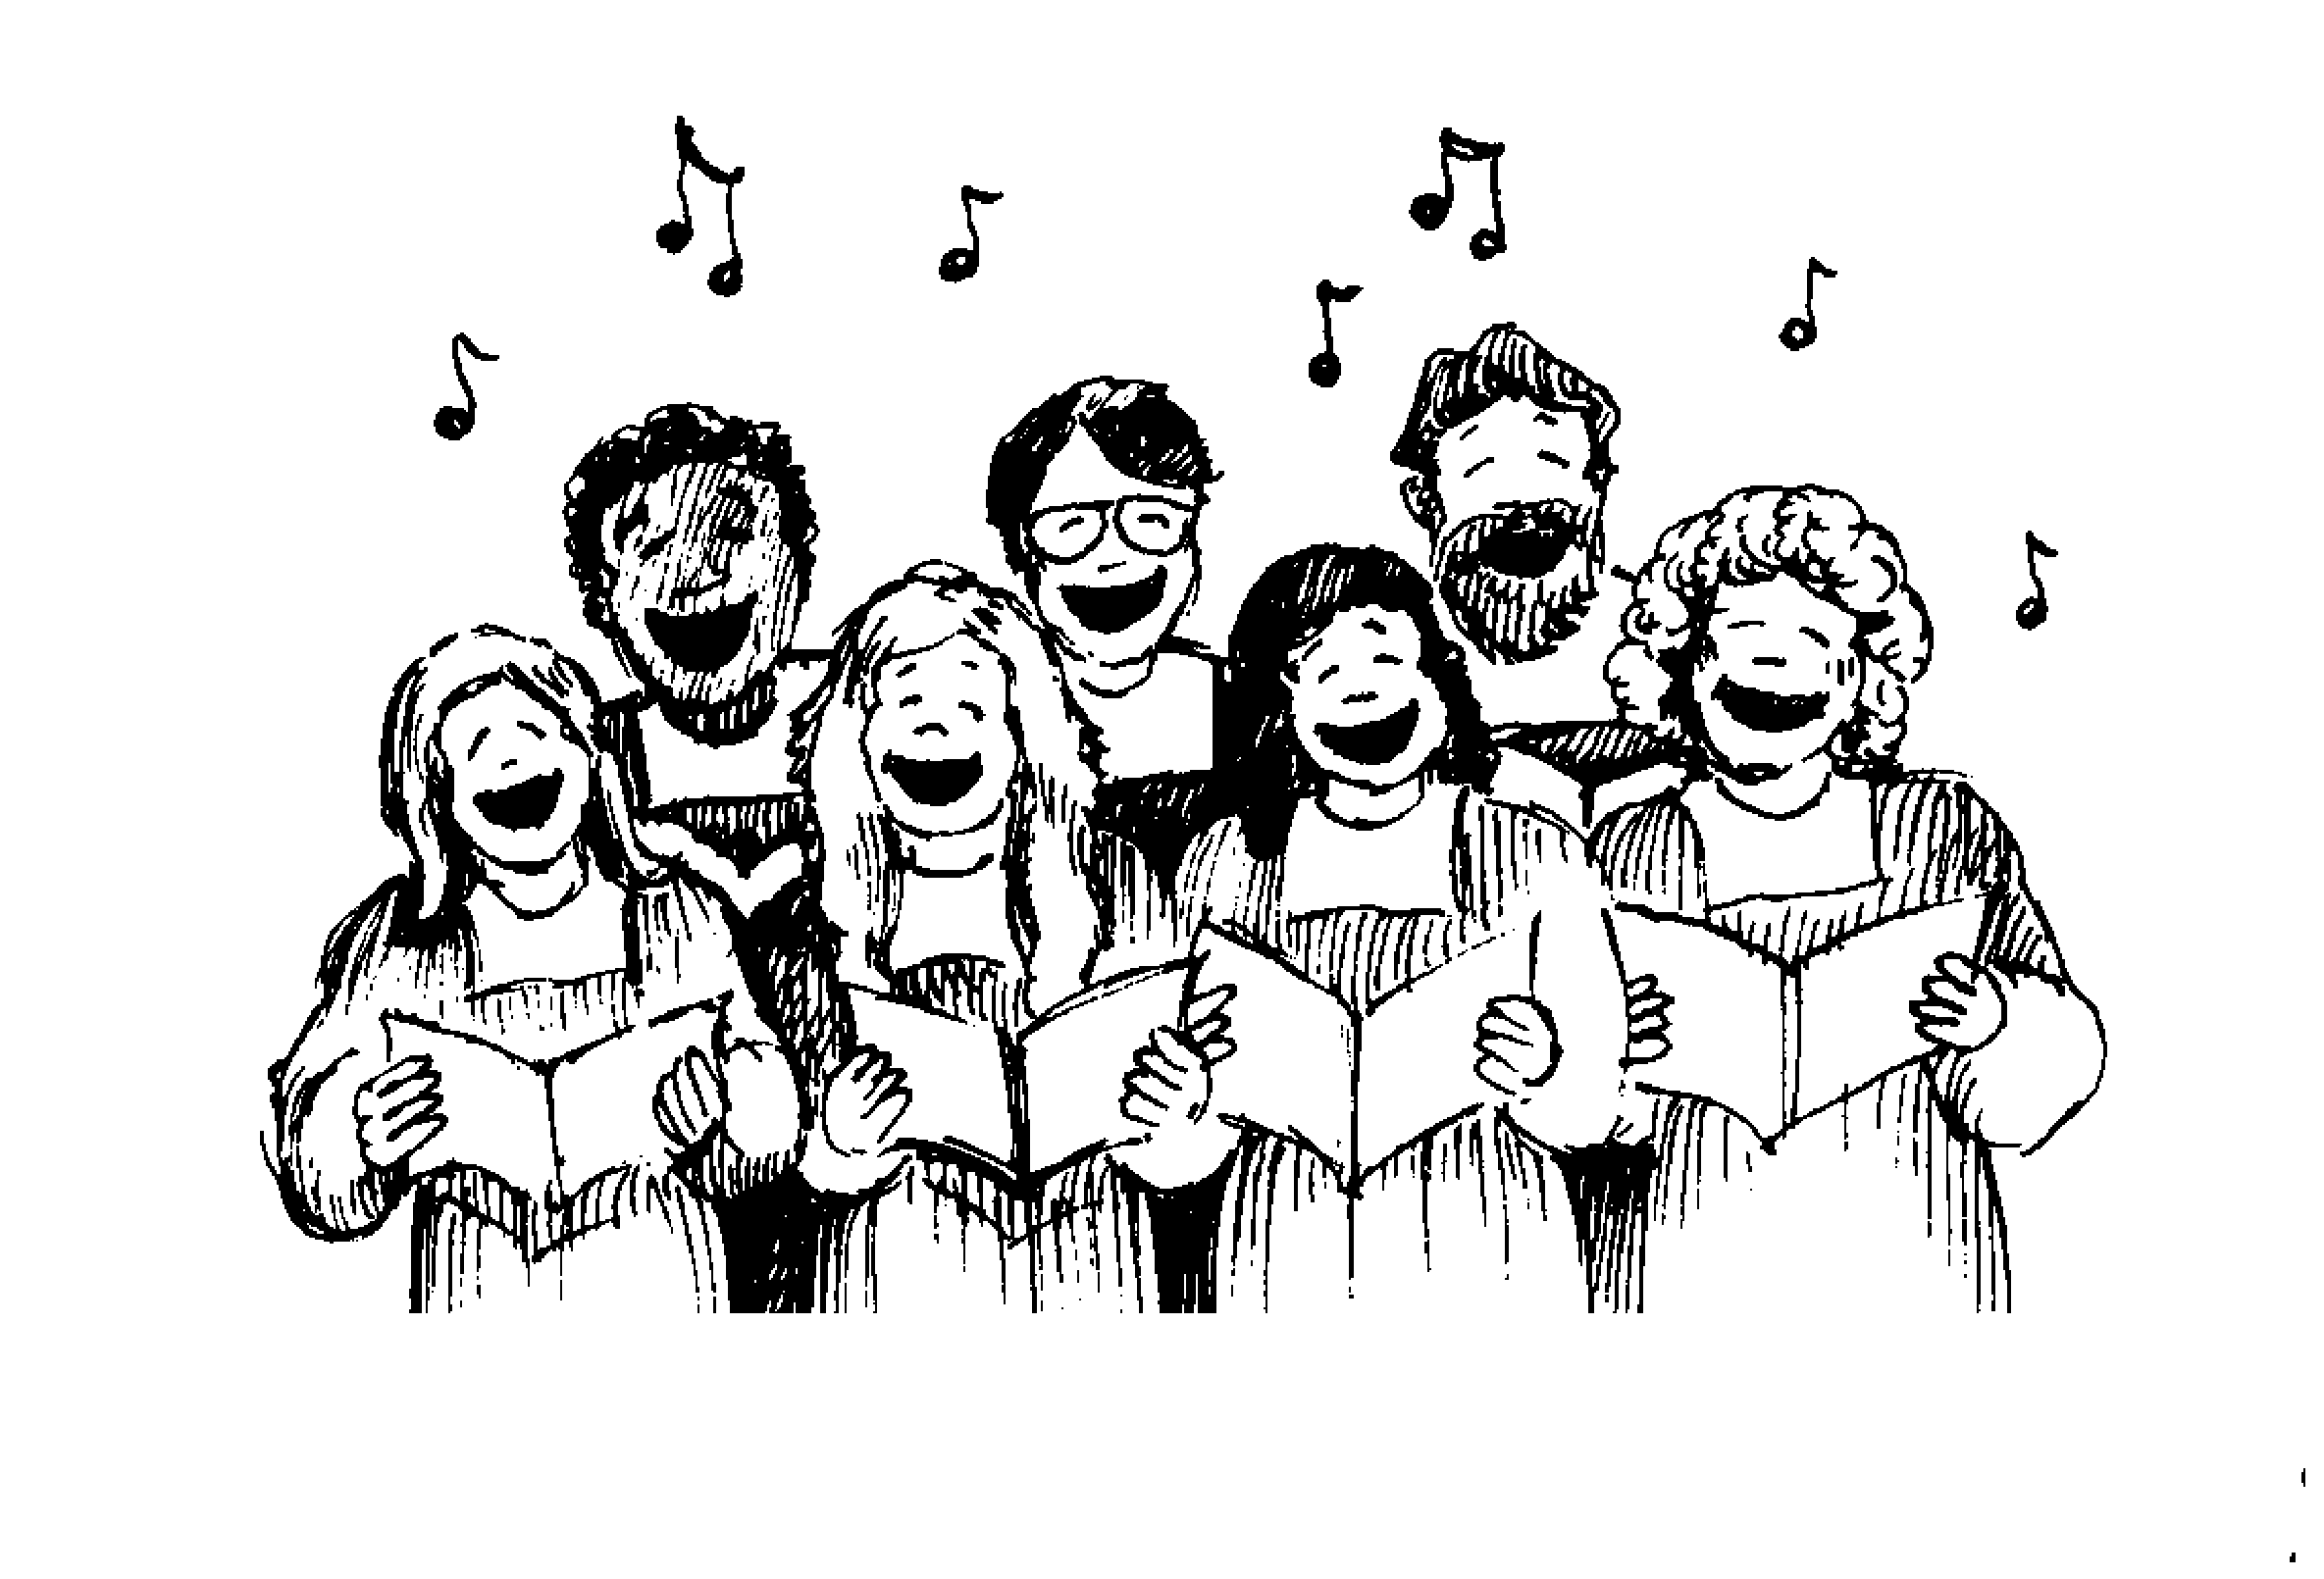
\includegraphics[scale=0.2]{choir01}
\end{center}



\end{document}